\documentclass[a4paper]{book}
\usepackage{graphicx}
\title{\LARGE{Calculus Quick Reference}}
\author{Sourav Datta}
\date{}
\begin{document}
\maketitle

\part{Before Calculus}

\chapter{Some Useful Algebraic Formulas}

\section{Arithmetic and Geometric Progressions}
Let $S$ be the sum of a series and $l$ be the last element of the series. 
For the Arithmetic Progression for a series of $n$ terms starting with $a$ and having a difference between the terms $n+1$ and $n$ denoted as $t_{n+1} = t_{n} + d$
\begin{equation}
S = \frac{n}{2}[2a + (n - 1)d]
\end{equation}
\begin{equation}
l = a + (n - 1)d
\end{equation}
Special case when $a = 1$ and $d = 1$,
\begin{equation}
S = \frac{n}{2}(n + 1)
\end{equation}
\begin{equation}
l = n
\end{equation}
For the Geometric Progression for a series of $n$ terms starting with $a$ and having a difference between the terms $n+1$ and $n$ denoted as $t_{n+1} = t_{n}r$
\begin{equation}
S = \frac{a(r^{n} - 1)}{r - 1}
\end{equation}
\begin{equation}
S = \frac{a(1 - r^{n})}{1 - r}
\end{equation}
\begin{equation}
l = ar^{n - 1}
\end{equation}

\section{Roots of Quadratic Equations}
The roots of a quadratic equation of the form $ax^{2} + bx + c = 0$ is given by,
\begin{equation}
x = \frac{-b \pm \sqrt{b^{2} - 4ac}}{2a}
\end{equation}
Properties of the roots
\begin{description}
\item If $b^{2} - 4ac$ is $positive$, roots are real and unequal.
\item If $b^{2} - 4ac$ is $0$, roots are real and equal ($= \frac{b}{2a}$).
\item If $b^{2} - 4ac$ is $negative$, roots are imaginary and unequal.
\item If $b^{2} - 4ac$ is $perfect square$, roots are rational and unequal.
\end{description}


\section{Permutations and Combinations}
\textbf{Permutation} is the process of $arranging$ some or all elements from a set. \textbf{Combination} is the $grouping$ or $selection$ of some or all elements from a set. 
\begin{enumerate}
\item If an operation can be performed $m$ ways and another operation can be performed $n$ ways, then the number of ways the two operation can be performed (in any order) is $mn$.
\item Find the $Permutations$ of n $unique$ elements taken $r$ at a time
\begin{equation}
^{n}P_{r} = n(n - 1)(n - 2)...(n - r + 1)
\end{equation}
\item Find the $Combinations$ of n $unique$ elements taken $r$ at a time
\begin{equation}
^{n}C_{r} = \frac{n!}{r!(n - r)!}
\end{equation}
\item The number of combinations of $n$ elements taken $r$ at a time is equal to number of combinations of $n$ elements taken $n - r$ at a time. This is called complementary combination
\begin{equation}
^{n}C_{r} = {}^{n}C_{n - r}
\end{equation}
\item The number of ways $m + n$ $unique$ objects can be divided in $m$ and $n$ groups
\begin{equation}
N_{m,n} = \frac{(m + n)!}{m!n!}
\end{equation}
If $m = n$, then
\begin{equation}
N_{m,n} = \frac{(m + n)!}{m!m!2!}
\end{equation}
\item The number of ways $m + n + p$ $unique$ objects can be divided in $m$, $n$ and $p$ groups
\begin{equation}
N_{m,n,p} = \frac{(m + n + p)!}{m!n!p!}
\end{equation}
If $m = n = p$, then
\begin{equation}
N_{m,n,p} = \frac{(m + n + p)!}{m!m!p!3!}
\end{equation}
\item The number of ways $n$ objects can be $arranged$ among themselves, where $p$ objects are of one kind, $q$ objects are another kind, $r$ objects are of third kind and rest are different 
\begin{equation}
x = \frac{n!}{p!q!r!}
\end{equation}
\end{enumerate}

\section{Binomial Theorem}
Binomial theorem for a constant $a$ and any index $n$ is defined as,
\begin{equation}
(x + a)^{n} = x^{n} + {}^{n}C_{1}ax^{n - 1} + {}^{n}C_{2}a^{2}x^{n - 2} + ... + {}^{n}C_{n}a^{n}
\end{equation}

\section{Inequalities}
\begin{description}
\item If $a < b$ then,
\begin{equation}
a + c < b + c
\end{equation}
\begin{equation}
a - c < b - c
\end{equation}
when $c > 0$
\begin{equation}
ac < bc
\end{equation}
\begin{equation}
\frac{a}{c} < \frac{b} {c}
\end{equation}
when $c < 0$,
\begin{equation}
ac > bc
\end{equation}
\begin{equation}
\frac{a}{c} > \frac{b} {c}
\end{equation}

\item If $a > b$ then,
\begin{equation}
a + c > b + c
\end{equation}
\begin{equation}
a - c > b - c
\end{equation}
when $c > 0$
\begin{equation}
ac > bc
\end{equation}
\begin{equation}
\frac{a}{c} > \frac{b} {c}
\end{equation}
when $c < 0$,
\begin{equation}
ac < bc
\end{equation}
\begin{equation}
\frac{a}{c} < \frac{b} {c}
\end{equation}
\item If $a > b$
\begin{equation}
-a < -b
\end{equation}
\item If $a < b$
\begin{equation}
-a > -b
\end{equation}
\end{description}
The same inequalities hold when the signs contain an equal component as well.


\chapter{Trigonometry}
This chapter briefly reviews the basics of Trigonometry. Calculus applied on Trigonometry will be discussed in later chapters.

\section{Basic Definitions}

\setlength\fboxrule{0pt}
\fbox{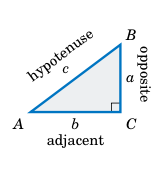
\includegraphics[scale=0.75]{trig1}}

Let angle $BAC$ be $\theta$, then

\begin{description}
\item \begin{equation} \sin \theta = \frac{a}{c} \end{equation}
\item \begin{equation} \cos \theta = \frac{b}{c} \end{equation}
\item \begin{equation} \tan \theta = \frac{a}{b} \end{equation}
\item \begin{equation} \csc \theta = \frac{c}{a} = \frac{1}{\sin \theta} \end{equation}
\item \begin{equation} \sec \theta = \frac{c}{b} = \frac{1}{\cos \theta} \end{equation}
\item \begin{equation} \cot \theta = \frac{c}{b} = \frac{1}{\tan \theta} \end{equation}
\end{description}

Trigonometric formulas for any angle on the Cartesian plane

\setlength\fboxrule{0pt}
\fbox{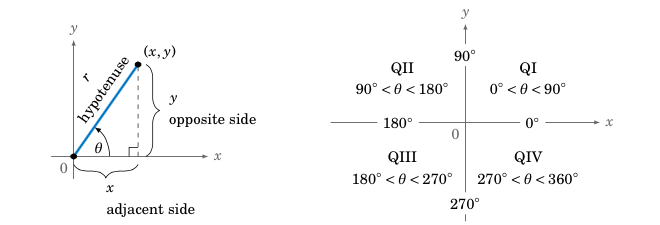
\includegraphics[scale=0.5]{trig2}}

\begin{description}
\item \begin{equation} \sin \theta = \frac{y}{r} \end{equation}
\item \begin{equation} \cos \theta = \frac{x}{r} \end{equation}
\item \begin{equation} \tan \theta = \frac{y}{x} \end{equation}
\item \begin{equation} \csc \theta = \frac{r}{y} = \frac{1}{\sin \theta} \end{equation}
\item \begin{equation} \sec \theta = \frac{r}{x} = \frac{1}{\cos \theta} \end{equation}
\item \begin{equation} \cot \theta = \frac{x}{y} = \frac{1}{\tan \theta} \end{equation}
\end{description}

Signs of trigonometric formulas in 4 quadrants

\setlength\fboxrule{0pt}
\fbox{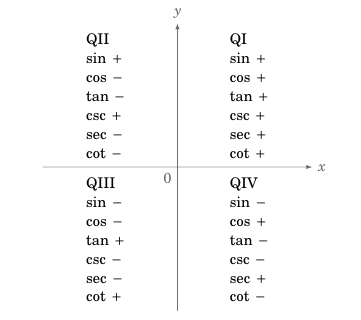
\includegraphics[scale=0.5]{trig3}}

Various properties of the trigonometric identities
\begin{description}
\item \begin{equation} \sin(\theta + \frac{\pi}{2}) = \cos \theta \end{equation}
\item \begin{equation} \cos(\theta + \frac{\pi}{2}) = -\sin \theta \end{equation}
\item \begin{equation} \tan(\theta + \frac{\pi}{2}) = -\cot \theta \end{equation}
\item \begin{equation} \sin(\theta - \frac{\pi}{2}) = -\cos \theta \end{equation}
\item \begin{equation} \cos(\theta - \frac{\pi}{2}) = \sin \theta \end{equation}
\item \begin{equation} \tan(\theta - \frac{\pi}{2}) = -\cot \theta \end{equation}
\item \begin{equation} \sin(\theta \pm \pi) = -\sin \theta \end{equation}
\item \begin{equation} \cos(\theta \pm \pi) = -\cos \theta \end{equation}
\item \begin{equation} \tan(\theta \pm \pi) = \tan \theta \end{equation}
\item \begin{equation} \sin(-\theta) = -\sin\theta \end{equation}
\item \begin{equation} \cos(-\theta) = \cos \theta \end{equation}
\item \begin{equation} \tan(-\theta) = -\tan \theta \end{equation}
\item \begin{equation} \sin(\frac{\pi}{2} - \theta) = \cos \theta \end{equation}
\item \begin{equation} \cos(\frac{\pi}{2} - \theta) = \sin \theta \end{equation}
\item \begin{equation} \tan(\frac{\pi}{2} - \theta) = \cot \theta \end{equation}
\item \begin{equation} \sin(\pi - \theta) = \sin \theta \end{equation}
\item \begin{equation} \cos(\pi - \theta) = -\cos \theta \end{equation}
\item \begin{equation} \tan(\pi - \theta) = -\tan \theta \end{equation}
\end{description}

\section{Laws of General Triangles}

\setlength\fboxrule{0pt}
\fbox{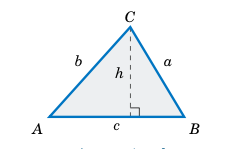
\includegraphics[scale=0.5]{trig4}}

\textbf{Law of Sine}
\begin{equation}
\frac{a}{\sin A} = \frac{b}{\sin B} = \frac{c}{\sin C}
\end{equation}

\textbf{Laws of Cosine}
\begin{equation}
a^2 = b^2 + c^2 - 2bc\cos A
\end{equation}
\begin{equation}
b^2 = c^2 + a^2 - 2ca\cos B
\end{equation}
\begin{equation}
c^2 = a^2 + b^2 - 2ab\cos C
\end{equation}

\textbf{Laws of Tangents}
\begin{equation}
\frac{a - b}{a + b} = \frac{\tan \frac{A - B}{2}}{\tan \frac{A + B}{2}}
\end{equation}
\begin{equation}
\frac{b - c}{b + c} = \frac{\tan \frac{B - C}{2}}{\tan \frac{B + C}{2}}
\end{equation}
\begin{equation}
\frac{c - a}{c + a} = \frac{\tan \frac{C - A}{2}}{\tan \frac{C + A}{2}}
\end{equation}

\textbf{Mollweide's equations}
\begin{equation}
\frac{a - b}{c} = \frac{\sin \frac{A - B}{2}}{\cos \frac{C}{2}}
\end{equation}
\begin{equation}
\frac{a + b}{c} = \frac{\cos \frac{A - B}{2}}{\sin \frac{C}{2}}
\end{equation}

\section{Basic Trigonometric Identities}
\begin{description}
\item \begin{equation}  \sin^2 \theta + \cos^2 \theta  = 1  \end{equation}
\item \begin{equation} -1 \le \sin \theta \le 1 \end{equation}
\item \begin{equation} -1 \le \cos \theta \le 1 \end{equation}
\item \begin{equation} 1 + \tan^2 \theta = \sec^2 \theta \end{equation}
\item \begin{equation} \cot^2 \theta + 1 = \csc^2 \theta \end{equation}
\end{description}

\section{Sums and Differences}
\begin{description}
\item \begin{equation} \sin (A + B) = \sin A \cos B + \cos A \sin B \end{equation}
\item \begin{equation} \cos (A + B) = \cos A \cos B - \sin A \sin B \end{equation}
\item \begin{equation} \sin (A - B) = \sin A \cos B - \cos A \sin B \end{equation}
\item \begin{equation} \cos (A - B) = \cos A \cos B + \sin A \sin B \end{equation}
\item \begin{equation} \tan (A + B) = \frac{\tan A + \tan B}{1 - \tan A \tan B} \end{equation}
\item \begin{equation} \tan (A - B) = \frac{\tan A - \tan B}{1 + \tan A \tan B}  \end{equation}
\end{description}

\section{Double and Half Angles}
\begin{description}
\item \begin{equation} \sin 2\theta = 2 \sin \theta \cos \theta \end{equation}
\item \begin{equation} \cos 2\theta = \cos^2 \theta - \sin^2 \theta \end{equation}
\item \begin{equation} \cos 2\theta = 2\cos^2 \theta - 1  = 1 - 2 \sin^2 \theta \end{equation}
\item \begin{equation} \tan 2\theta = \frac{2 \tan \theta}{1 - \tan^2 \theta} \end{equation}
\item \begin{equation} \sin \frac{\theta}{2} = \pm \sqrt{\frac{1 - \cos \theta}{2}} \end{equation}
\item \begin{equation} \cos \frac{\theta}{2} = \pm \sqrt{\frac{1 + \cos \theta}{2}} \end{equation}
\item \begin{equation} \tan \frac{\theta}{2} = \pm \sqrt{\frac{1 - \cos \theta}{1 + \cos \theta}} \end{equation}
\end{description}

\section{Other Identities}
\begin{description}
\item \begin{equation} \sin A \cos B = \frac{1}{2} (\sin(A + B) + \sin(A - B)) \end{equation}
\item \begin{equation} \cos A \sin B = \frac{1}{2} (\sin(A + B) - \sin(A - B)) \end{equation}
\item \begin{equation} \cos A \cos B = \frac{1}{2} (\cos(A + B) + \cos(A - B)) \end{equation}
\item \begin{equation} \sin A \sin B = -\frac{1}{2} (\cos(A + B) - \cos(A - B)) \end{equation}
\item \begin{equation} \sin A + \sin B = 2 \sin \frac{1}{2} (A+B) \cos \frac{1}{2}(A - B) \end{equation}
\item \begin{equation} \sin A - \sin B = 2 \cos \frac{1}{2} (A+B)  \sin \frac{1}{2}(A - B) \end{equation}
\item \begin{equation} \cos A + \cos B = 2 \cos \frac{1}{2} (A+B) \cos \frac{1}{2}(A - B) \end{equation}
\item \begin{equation} \cos A - \cos B = -2 \sin \frac{1}{2} (A+B)  \sin \frac{1}{2}(A - B) \end{equation}
\end{description}

\section{Inverse Functions}
\begin{description}
\item \begin{equation} \sin^{-1}(\sin y) = y\ \ ,\ -\frac{\pi}{2} \le y \le \frac{\pi}{2} \end{equation}
\item \begin{equation} \sin(\sin^{-1} x) = x\ \ ,\ -1 \le x \le 1 \end{equation}
\item \begin{equation} \cos^{-1}(\cos y) = y\ \ ,\ 0 \le y \le \pi \end{equation}
\item \begin{equation} \cos^{-1}(\cos x) = x\ \ ,\ -1 \le x \le 1 \end{equation}
\end{description}

\end{document}
